\chapter[FESDData]{FESDData - Data Acquisition and Labelling of FESDDataset}
\label{sec:data_processing}

One of the most important aspects of machine learning is the data acquisition. In this thesis a custom tool is developed which is capapble of capturing and labelling multi-modal data. The tool is called \textbf{F}ault \textbf{E}stimator for \textbf{S}keleton \textbf{D}etection \textbf{Data} processor (FESDData). The tool is capapable of capturing RGBD data from multiple different RGBD cameras as well as pose data calculated by Nuitrack. Nuitrack which was developed by 3DiVi Inc\footnote{\url{https://nuitrack.com/}} it was chosen as the pose estimation backbone, since it provided the support of multiple different cameras as well as the ability to record the pose data simultaneously. 

Additionally to Nuitrack, FESDData is capable of calculating the pose information using OpenPose after the recording is done. This offers future support for other pose estimation backbones. However, OpenPose is not used in the scope of this thesis.

FESDData is designed to be easy to use and to require minimal setup. The tool is designed to be used by anyone and to be used without much need for setup or tweaking. It allows for the rapid capture of RGBD datasets with pre-labeling of multiple different recordings. The parameters can be adapted to capture datasets for many different application, e.g. Action detection. 

For this thesis exercises have been derived which are designed to emulate different scenarios with different difficulties. These exercises are discussed in section \ref{sec:errors}. The labelling of errors in the data requires domain specific knowledge and is therefore done manually. The resulting dataset, FESDDataset, is discussed in section \ref{sec:dataset}. It consists of the RGBD data as well as the pose data and the labels for the errors for each of the joints in the pose.

In this chapter, the approach to the design of the exercises is discussed by showing the difficulties of human pose estimation. Furthermore, the data acquisition and labelling process is discussed. Finally, the dataset is presented.


\section{Challenges in Human Pose Estimation}
\label{sec:errors}
% include this in the dataset section rather
% cahllenges are already mentioned in the introduction so no need to go into detail here
In this chapter, possible faults and difficulties that occur during human pose estimation are discussed. These difficulties are caused by different factors, such as the environment, the camera, the person, and the software. 

These difficulties are important to understand, as they can cause the joints to be in the incorrect position or missing. This can cause the pose estimation to be incorrect, and therefore, the human-computer interaction will be hampered.

\subsection{Environment}

The environment in which the data is recorded is crucial to the quality of the pose estimation. The environment can be split into multiple categories, which are discussed in the following sections. The mentioned difficulties depend on how the method itself works. For example, if a method uses RGB data, the background might be an issue, whereas if a method uses depth data, the lighting is more of an issue.

\subsubsection{Background}

The background of the scene can cause difficulties in the human pose estimation process. Methods using RGB cameras might have difficulties detecting the difference between the foreground and the background. In RGB-D-based methods, the background can cause depth ambiguities which might even prevent the human from being detectable, especially if the background is reflective, or too close to the user.

\subsubsection{Lighting}

While RBG cameras are to some extent insensitive to the amount of incoming light, RGB-D cameras are highly influenced by the lighting. Most RGB-D cameras use infrared light to determine the depth of the scene, some use a pattern of infrared light that is projected onto the scene and distorted by physical objects and some use the time-of-flight method to determine the depth of the scene. The issue that arises with infrared light is that it is also emitted by the sun. This means that light emitted by the sun can interfere with the infrared light emitted by the camera. This can cause the depth of the scene to be incorrect or missing in parts with a high intensity of sunlight.

To reduce the effect of the sunlight, the camera can be placed in a room with curtains or blinds. This will reduce the amount of sunlight that enters the room and therefore reduce the effect of the sunlight on the camera. Since lighting is hard to perfectly reproduce without a controlled environment, the lighting is not varied throughout the experiments. Therefore, all of the experiments were conducted in a room without any natural light or during the night.

However, if a method heavily relies on RGB data for the pose estimation, eliminating any form of light is not a valid option since then the data that can be gathered by RGB cameras in low light environments is limited and may result in a wrong pose.

\subsubsection{Objects}

The objects in the scene may cause issues in the human pose estimation process if they either occlude the user or are too close to the user. Occlusion can cause inaccurate or missing joints. Whereas objects that are too close to the user can cause joints to move to these objects instead.

\subsubsection{Chair}

If the exercise is performed in a sitting position the chair might influence the accuracy of HPE. For example, wheelchairs pose a problem in some estimators but a significant part of users who use pose estimation for rehabilitation games are using wheelchairs due to health conditions. Furthermore, bulky chairs that go higher than the head may prevent accurate head detection and
 silhouette estimation, which is also sometimes used instead of the pose.

\section{Camera}

In this section, $REPLACE_WE$ discuss the difficulties that can occur due to the camera. SilverFit uses a predefined camera setup, which is the same for every customer. This setup is tried and tested and has been used for many years. However, the camera setup can still cause difficulties during human pose estimation.

The two main difficulties that can occur with the camera setup are the camera position and the camera angle. Additionally, the camera itself can make the pose estimation process more difficult.

\subsection{Distance}

The distance of the camera to the user effects the quality of the pose estimation in multiple ways. Firstly, if the user is too close to the camera, the camera might not get the complete body into frame. The legs and arms might be off the frame preventing them to be estimated properly. Additionally, depth cameras can only detect the depth for a specific range, so if a user is too close they might not be visible to the depth camera.

However, if the user is too far away from the camera, the person might be too small to be detected reliably. There are methods which can detect a human pose from a far distance, however, the further away people get from a camera the more challenging it is. Additionally, as mentioned before, depth cameras operate at different depth ranges. If a user is too far away from the camera it wont be visible to the depth camera. This range varies from camera to camera and also depends on the method of detection.

\subsection{Angle}

When considering angles the main focus lays on pitch and roll. For the experiments the yaw is assumed as fixed and directed facing the user, such that the user is in the center. Most human pose estimators are trained without roll in mind. The cameras are usually setup so that any roll is minimised.

Additionally, the pitch may introduce or reduce the occlusion of joints by other joints. It also influences which area is best for human pose estimation. The pitch of a camera depends on what the main application is. For example, if the legs are not considered then the pitch could be used to focus more on the upper body.

\subsection{Resolution}

The resolution of the camera, or rather the resolution of the image captured by the camera influences the information that can be gathered about the human and therefore influence the performance of the pose estimation. Also here the application and specifically range are important for choosing the right resolution. If a user is far away a higher resolution is needed to detect the pose reliably.

This is also the case for RGBD cameras. Most RGBD cameras have a set range at which they operate. Additionally, the further away from a depth camera you get, the more noisy the depth stream becomes.
\subsection{Person}

Finally, one of the main error sources of human pose estimation is the person. The person can cause difficulties in the human pose estimation process by moving, wearing specific clothes, or having a different body posture. Body posture is of special importance for SilverFit since SilverFit specialises in games for rehabilitation and elderly people. Elderly people have different body postures than the average person, which can cause difficulties in the human pose estimation process.

\subsubsection{Clothes}

As mentioned earlier, most RGBD cameras use infrared light to determine the depth of the scene. This means that the clothes of the user can cause more or less absorption of light and therefore influence the detected depth. This can cause the joints to be detected in the wrong position or not at all. This is especially the case for dark clothes, as they absorb more light than light clothes.

Furthermore, bulky clothes or skirts and dresses may influence the pose, since the exact position of the legs is not visible.

\subsubsection{Training Equipment}

To make exercises more challenging some physiotherapists use additional training equipment. This could be weights that are held in the hand or weights that are attached to the ankles. These weights change the outline of the body and therefore influence the pose estimation. 

\subsubsection{Exercises}
\label{sec:exercises}

Finally, the most important factor is the exercise that is carried out. In this section, both exercises that are easy to detect as well as some exercises that are difficult to detect are proposed.

These exercises might not be the most realistic, but they represent common issues with pose estimation in a reproducible manner. Furthermore, these exercises are not too difficult to perform, which makes them suitable for testing the pose estimators. The difficulty rating of the exercise might not reflect the difficulty of the exercise for the user, but it does reflect the difficulty of the exercise for the pose estimator.

The exercises are numbered according to the difficulty. The first letter is an identifier that is an exercise. The first digit indicates the difficulty of the exercise, while the second digit indicates the number of the exercise. The difficulty is rated from 0 to 4, where 0 is the easiest and 4 is the most difficult. The exercises are divided into four categories: trivial, easy, medium and hard.

\paragraph{Trivial Exercises}

Trivial exercises are exercises that are easy to detect and are therefore good for testing the pose estimators. These exercises are not too difficult to detect and are therefore good for testing the pose estimators. The exercises do not involve any movement, which makes detecting the joints easier. The two trivial exercises can be seen in table \ref{tab:trivial_exercises}. Example images of the exercises can be seen in figure \ref{fig:trivial_exercises}.

\begin{table}[ht]
  \caption[Trivial Exercises]{The two Trivial Exercises, E-0.00 and E-0.01.}
  \label{tab:trivial_exercises}
  \begin{tabular}{p{0.1\linewidth}p{0.3\linewidth}p{0.55\linewidth}}
  \hline
  Exercise & Short Description         & challenge   \\ \hline
  E-0.00   & Arms hanging to the side  & This exercise is very easy since no part of the body is occluded by any other part. Additionally, the joints are not moving. \\
  E-0.01   & Arms extended to the side & The arms are no longer in a natural position but still not occluded and no joint is moving \\ \hline
  \end{tabular}
\end{table} 



\begin{figure}[ht]
  \centering
  \begin{subfigure}[b]{0.16\linewidth}
      \centering
      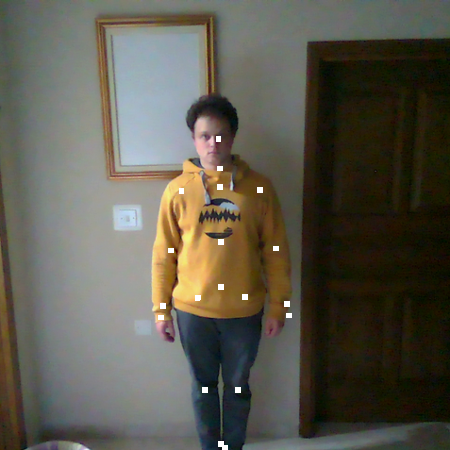
\includegraphics[width=\textwidth]{figures/samples/trivial/E-0.00_10.png}
      \caption[]{E-0.00}
  \end{subfigure}
  \hfill
  \begin{subfigure}[b]{0.16\linewidth}
      \centering
      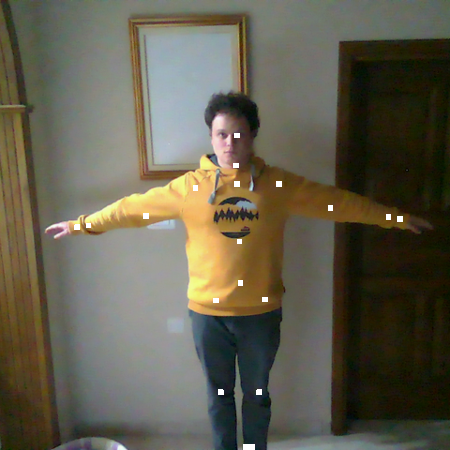
\includegraphics[width=\textwidth]{figures/samples/trivial/E-0.01_38.png}
      \caption[]{E-0.01}
  \end{subfigure}
  \caption[Trivial Exercises]{The two trivial exercises. (a) Arms hanging to the side. (b) Arms extended to the side.}
  \label{fig:trivial_exercises}
\end{figure}  

\paragraph{Easy Exercises}

Easy exercises are essential for creating a good baseline of how the pose estimators should work. These exercises are not too difficult to detect and are therefore good for testing the pose estimators. The exercises include no self-occlusion and are recorded in a standing position, which is generally the easiest position to detect. The easy exercises can be seen in table \ref{tab:easy_exercises}. Example images of the exercises can be seen in figure \ref{fig:easy_exercises}.

\begin{table}[ht]
  \caption[Easy Exercises]{The Easy exercises, E-1.00 through E-1.03. The easy exercises include both standing and sitting exercises.}
  \label{tab:easy_exercises}
  \begin{tabular}{p{0.1\linewidth}p{0.3\linewidth}p{0.55\linewidth}}
  \hline
  Exercise & Short Description             & Challenge \\ \hline
  E-1.00   & Raising the arms to the side  & Now the arms are no longer stationary. Still, there is no Occlusion. \\
  E-1.01   & Raising the arms to the front & The arms might occlude themselves and part of the body.  \\
  E-1.02   & Raise the knees to the chest  & The legs now occlude parts of the hip.  \\
  E-1.03   & Sit in a chair motionless     & Sitting positions are more challenging to detect than standing positions since there is now a chair in the background and the body occludes itself.\\ \hline
  \end{tabular}
  \end{table}



  \begin{figure}[ht]
    \centering
    \begin{subfigure}[b]{0.16\linewidth}
        \centering
        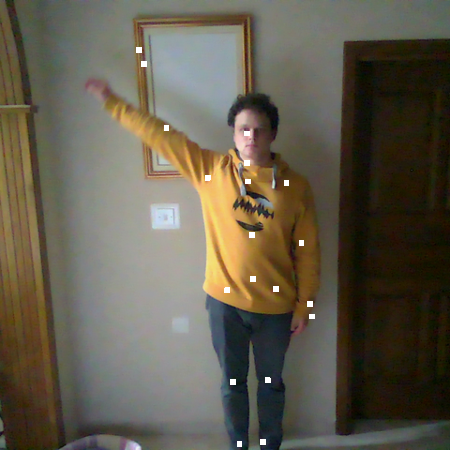
\includegraphics[width=\textwidth]{figures/samples/easy/E-1.00_126.png}
        \caption[]{E-1.00}
    \end{subfigure}
    \hfill
    \begin{subfigure}[b]{0.16\linewidth}
        \centering
        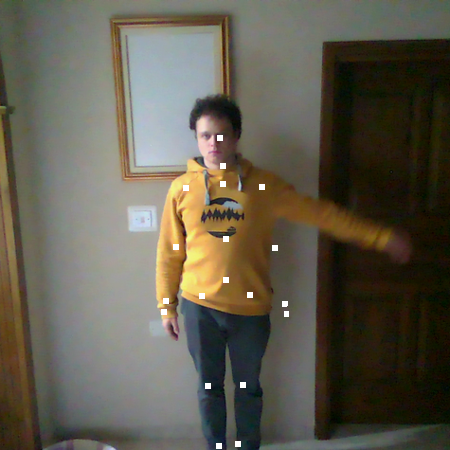
\includegraphics[width=\textwidth]{figures/samples/easy/E-1.00_137.png}
        \caption[]{E-1.00}
    \end{subfigure}
    \hfill
    \begin{subfigure}[b]{0.16\linewidth}
        \centering
        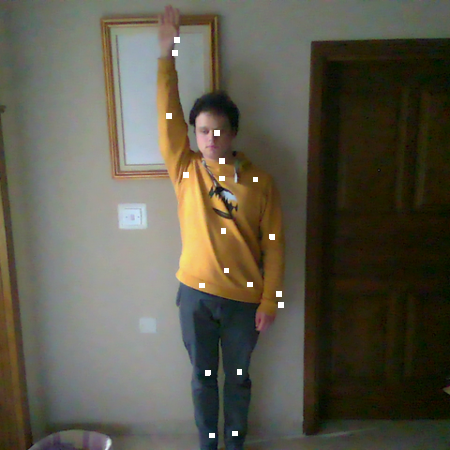
\includegraphics[width=\textwidth]{figures/samples/easy/E-1.01_188.png}
        \caption[]{E-1.01}
    \end{subfigure}
    \hfill
    \begin{subfigure}[b]{0.16\linewidth}
        \centering
        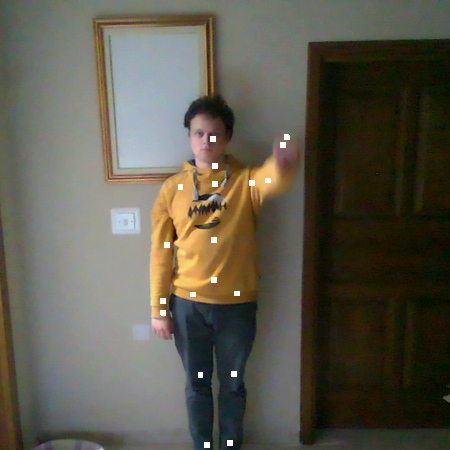
\includegraphics[width=\textwidth]{figures/samples/easy/E-1.01_197.png}
        \caption[]{E-1.01}
    \end{subfigure}
    \hfill
    \begin{subfigure}[b]{0.16\linewidth}
        \centering
        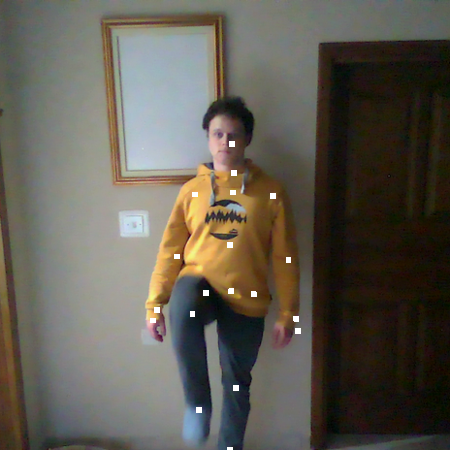
\includegraphics[width=\textwidth]{figures/samples/easy/E-1.02_230.png}
        \caption[]{E-1.02}
    \end{subfigure}
    \hfill
    \begin{subfigure}[b]{0.16\linewidth}
        \centering
        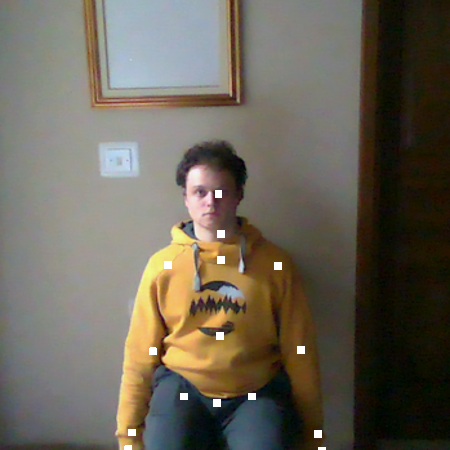
\includegraphics[width=\textwidth]{figures/samples/easy/E-1.03_301.png}
        \caption[]{E-1.03}
    \end{subfigure}
    \caption[Easy Exercises]{The four easy exercises. (a) Raising the arms to the side. (b) Raising the arms to the front. (c) Raising the knee up to the chest. (d) Sitting in a chair motionless.}
    \label{fig:easy_exercises}
  \end{figure}  

\paragraph{Medium Exercises}

Exercises which are performed in a seated position are harder to detect since parts of the body are occluded. Medium exercises focus on exercises, which are performed in a seated position. The medium exercises can be seen in table \ref{tab:medium_exercises}. Example images of the exercises can be seen in figure \ref{fig:medium_exercises}.

\begin{table}[ht]
  \caption[Medium Exercises]{The Medium exercises, E-2.00 through E-2.03. The medium exercises are all in a sitting position.}
  \label{tab:medium_exercises}
  \begin{tabular}{p{0.1\linewidth}p{0.3\linewidth}p{0.55\linewidth}}
  \hline
  Exercise & Short Description                                     & Challenge \\ \hline
  E-2.00   & Raising the arms to the side while sitting            & Now the arms are no longer stationary. With added difficulty since the user is now sitting.         \\
  E-2.01   & Raising the arms to the front while sitting           & The arms might occlude themselves and part of the body. Additionally, the person is now sitting down\\
  E-2.02   & Crossing the arms in front of the chest while sitting & The arms now occlude large parts of the upper body.                                                                                            \\
  E-2.03   & Raising the knee to the chest while sitting           & More parts of the upper body are occluded and not seen by the camera.                              \\ \hline
  \end{tabular}
  \end{table}



  \begin{figure}[ht]
    \centering
    \begin{subfigure}[b]{0.16\linewidth}
        \centering
        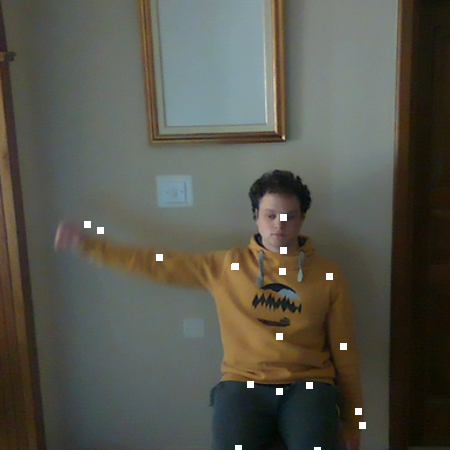
\includegraphics[width=\textwidth]{figures/samples/medium/E-2.00_365.png}
        \caption[]{E-2.00}
    \end{subfigure}
    \hfill
    \begin{subfigure}[b]{0.16\linewidth}
        \centering
        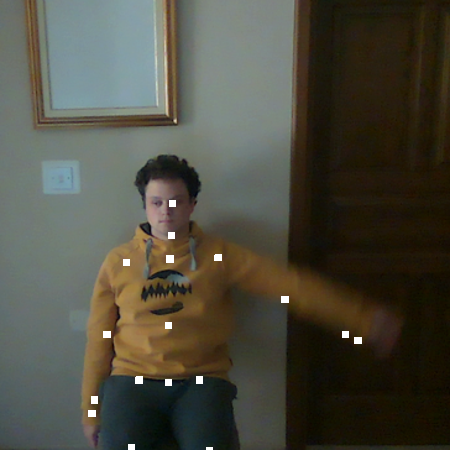
\includegraphics[width=\textwidth]{figures/samples/medium/E-2.00_385.png}
        \caption[]{E-2.00}
    \end{subfigure}
    \hfill
    \begin{subfigure}[b]{0.16\linewidth}
        \centering
        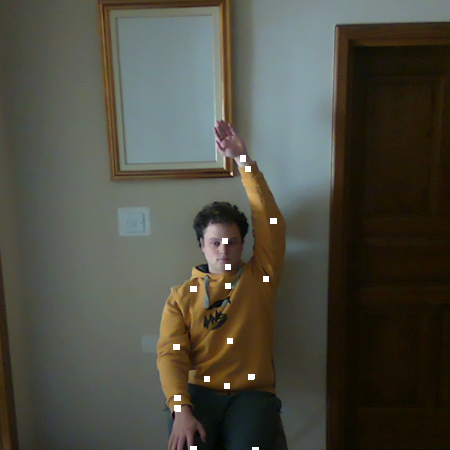
\includegraphics[width=\textwidth]{figures/samples/medium/E-2.01_440.png}
        \caption[]{E-2.01}
    \end{subfigure}
    \hfill
    \begin{subfigure}[b]{0.16\linewidth}
        \centering
        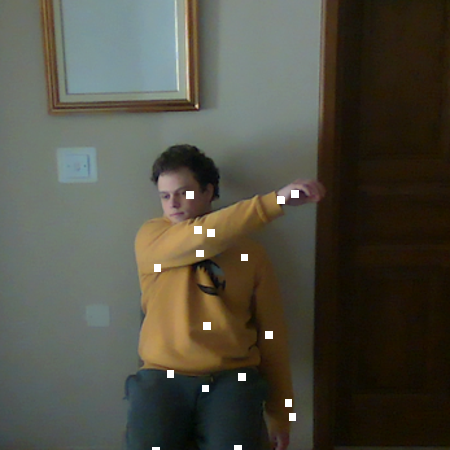
\includegraphics[width=\textwidth]{figures/samples/medium/E-2.02_487.png}
        \caption[]{E-2.02}
    \end{subfigure}
    \hfill
    \begin{subfigure}[b]{0.16\linewidth}
        \centering
        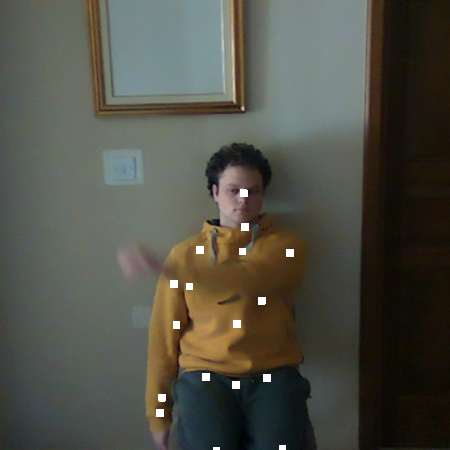
\includegraphics[width=\textwidth]{figures/samples/medium/E-2.02_500.png}
        \caption[]{E-2.02}
    \end{subfigure}
    \hfill
    \begin{subfigure}[b]{0.16\linewidth}
        \centering
        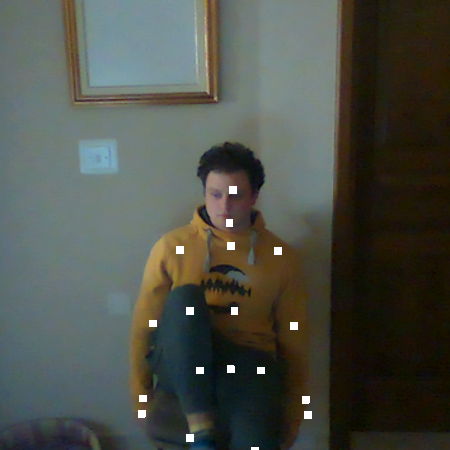
\includegraphics[width=\textwidth]{figures/samples/medium/E-2.03_590.png}
        \caption[]{E-2.03}
    \end{subfigure}
    \caption[Easy Exercises]{The four medium exercises. (a) Raising the arms to the side while sitting. (b) Raising the arms to the front while sitting. (c) Crossing the arms in front of the chest while sitting. (d) Raising the knee up to the chest while sitting.}
    \label{fig:medium_exercises}
  \end{figure}  

\paragraph{Difficult Exercises}

Difficult exercises are exercises that are performed in a standing position and involve leg movement. Leg joints are harder to detect than arm joints and therefore pose a greater challenge for the pose estimators. These exercises will be in a seating position and with a difficult posture, such as leaning forward. The difference in posture aims at creating a realistic representation of real-world exercises.

Tölgyessy et al. found that facing away from the camera decreases the accuracy of HPE due to self-occlusion. \cite{HPEIsHard} Therefore, some of the exercises will be performed facing away from the camera. The difficult exercises can be seen in table \ref{tab:difficult_exercises}. Example images of the exercises can be seen in figure \ref{fig:difficult_exercises}.

\begin{table}[ht]
  \caption[Difficult Exercises]{The Difficult exercises, E-3.00 through E-3.02. The difficult exercises are all in a standing position.}
  \label{tab:difficult_exercises}
  \begin{tabular}{p{0.1\linewidth}p{0.3\linewidth}p{0.55\linewidth}}
  \hline
  Exercise & Short Description                                                              & Challenge \\ \hline
  E-3.00   & Bowing toward the camera                                                       & The head is often used as an anchor point for the skeleton as it is quite stable. When bowing forward the head is no longer easily detectable. \\
  E-3.01   & Raising the knee leaning forward                                               & Leaning forward increases the difficulty since the position is not natural \\
  E-2.02   & Raising the knee leaning forward while sitting and facing away from the camera & Facing away from the camera makes it more difficult to detect the pose and induces more occlusion.  \\ \hline
  \end{tabular}
\end{table}



\begin{figure}[ht]
  \centering
  \begin{subfigure}[b]{0.16\linewidth}
      \centering
      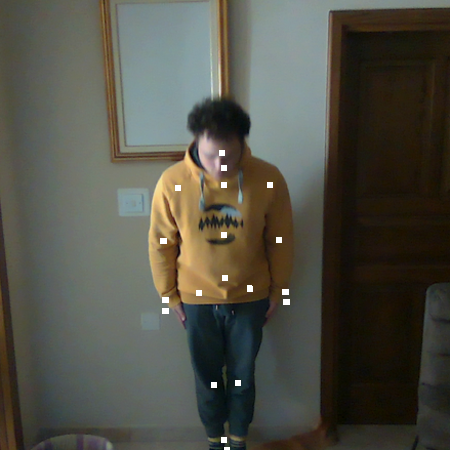
\includegraphics[width=\textwidth]{figures/samples/hard/E-3.00_530.png}
      \caption[]{E-3.00}
  \end{subfigure}
  \hfill
  \begin{subfigure}[b]{0.16\linewidth}
      \centering
      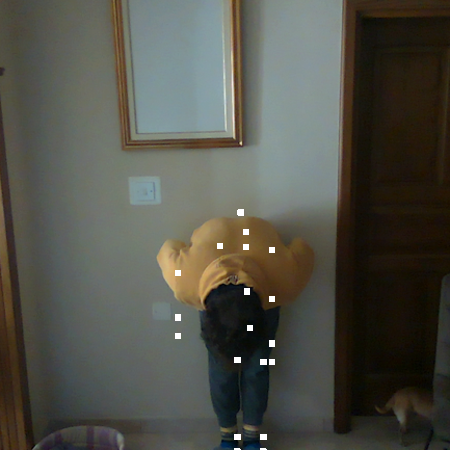
\includegraphics[width=\textwidth]{figures/samples/hard/E-3.00_535.png}
      \caption[]{E-3.00}
  \end{subfigure}
  \hfill
  \begin{subfigure}[b]{0.16\linewidth}
      \centering
      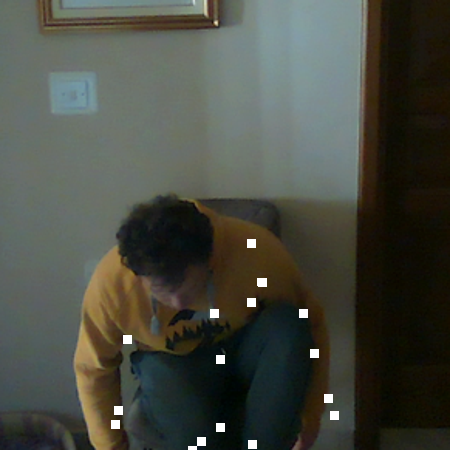
\includegraphics[width=\textwidth]{figures/samples/hard/E-3.01_635.png}
      \caption[]{E-3.01}
  \end{subfigure}
  \hfill
  \begin{subfigure}[b]{0.16\linewidth}
      \centering
      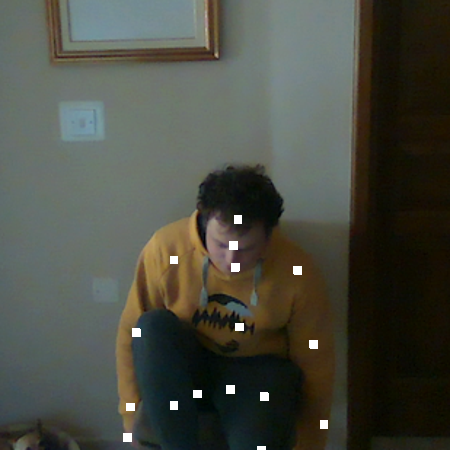
\includegraphics[width=\textwidth]{figures/samples/hard/E-3.01_685.png}
      \caption[]{E-3.01}
  \end{subfigure}
  \hfill
  \begin{subfigure}[b]{0.16\linewidth}
      \centering
      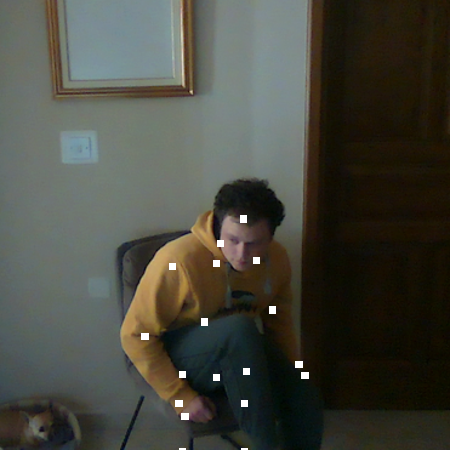
\includegraphics[width=\textwidth]{figures/samples/hard/E-3.02_695.png}
      \caption[]{E-3.02}
  \end{subfigure}
  \hfill
  \begin{subfigure}[b]{0.16\linewidth}
      \centering
      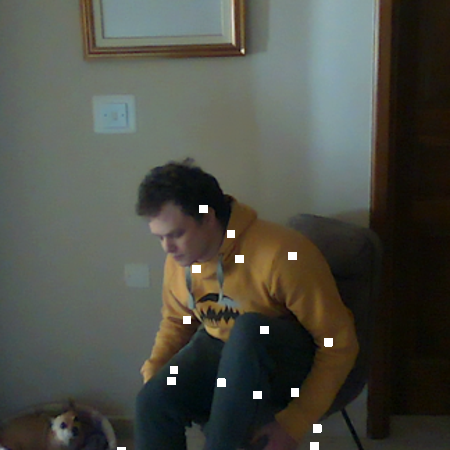
\includegraphics[width=\textwidth]{figures/samples/hard/E-3.02_725.png}
      \caption[]{E-3.02}
  \end{subfigure}
  \caption[Difficult Exercises]{The three difficult exercises. (a) Bowing toward the camera. (b) Raising the knee leaning forward. (c) Raising the knee leaning forward while sitting and facing away from the camera. Some of the exercises contain errors in the sample.}
  \label{fig:difficult_exercises}
\end{figure}

\section{Data acquisition}
\label{sec:data_acquisition}

Different modalities were captured to create a dataset that reproduces a real-world application of HPE for RGB-D cameras. The different modalities are RGB data, depth data, and joint data. While the Nuitrack SDK offers to capture the data from the RGB-D cameras and the joint data, the recorded files cannot, at the time of writing, be read without using the Nuitrack SDK. Therefore, FESDData, a custom RGB-D+HPE capturing and labelling tool was developed. 

FESDData has two main uses which are interlocked. Firstly, it allows capturing predefined, as well as custom, exercises repeatedly automatically making the capturing experience when capturing many different exercises with multiple repetitions more comfortable. Secondly, it allows reviewing and labelling the captured data with error labels. The lightweight nature of FESDData allows it to seamlessly capture both the RGB-D stream and the skeleton data at the same time while ensuring a stable fast framerate. The dataset that is used by FESDModel was captured at a framerate of 30 frames per second. The interface of FESDData can be seen in figure \ref{fig:fesddata}. On the left side of the image the interface can be seen and on the right, there is an example for data labelling of Exercise E1-02.


\begin{figure}
  \centering
  \begin{subfigure}[b]{0.49\linewidth}
      \centering
      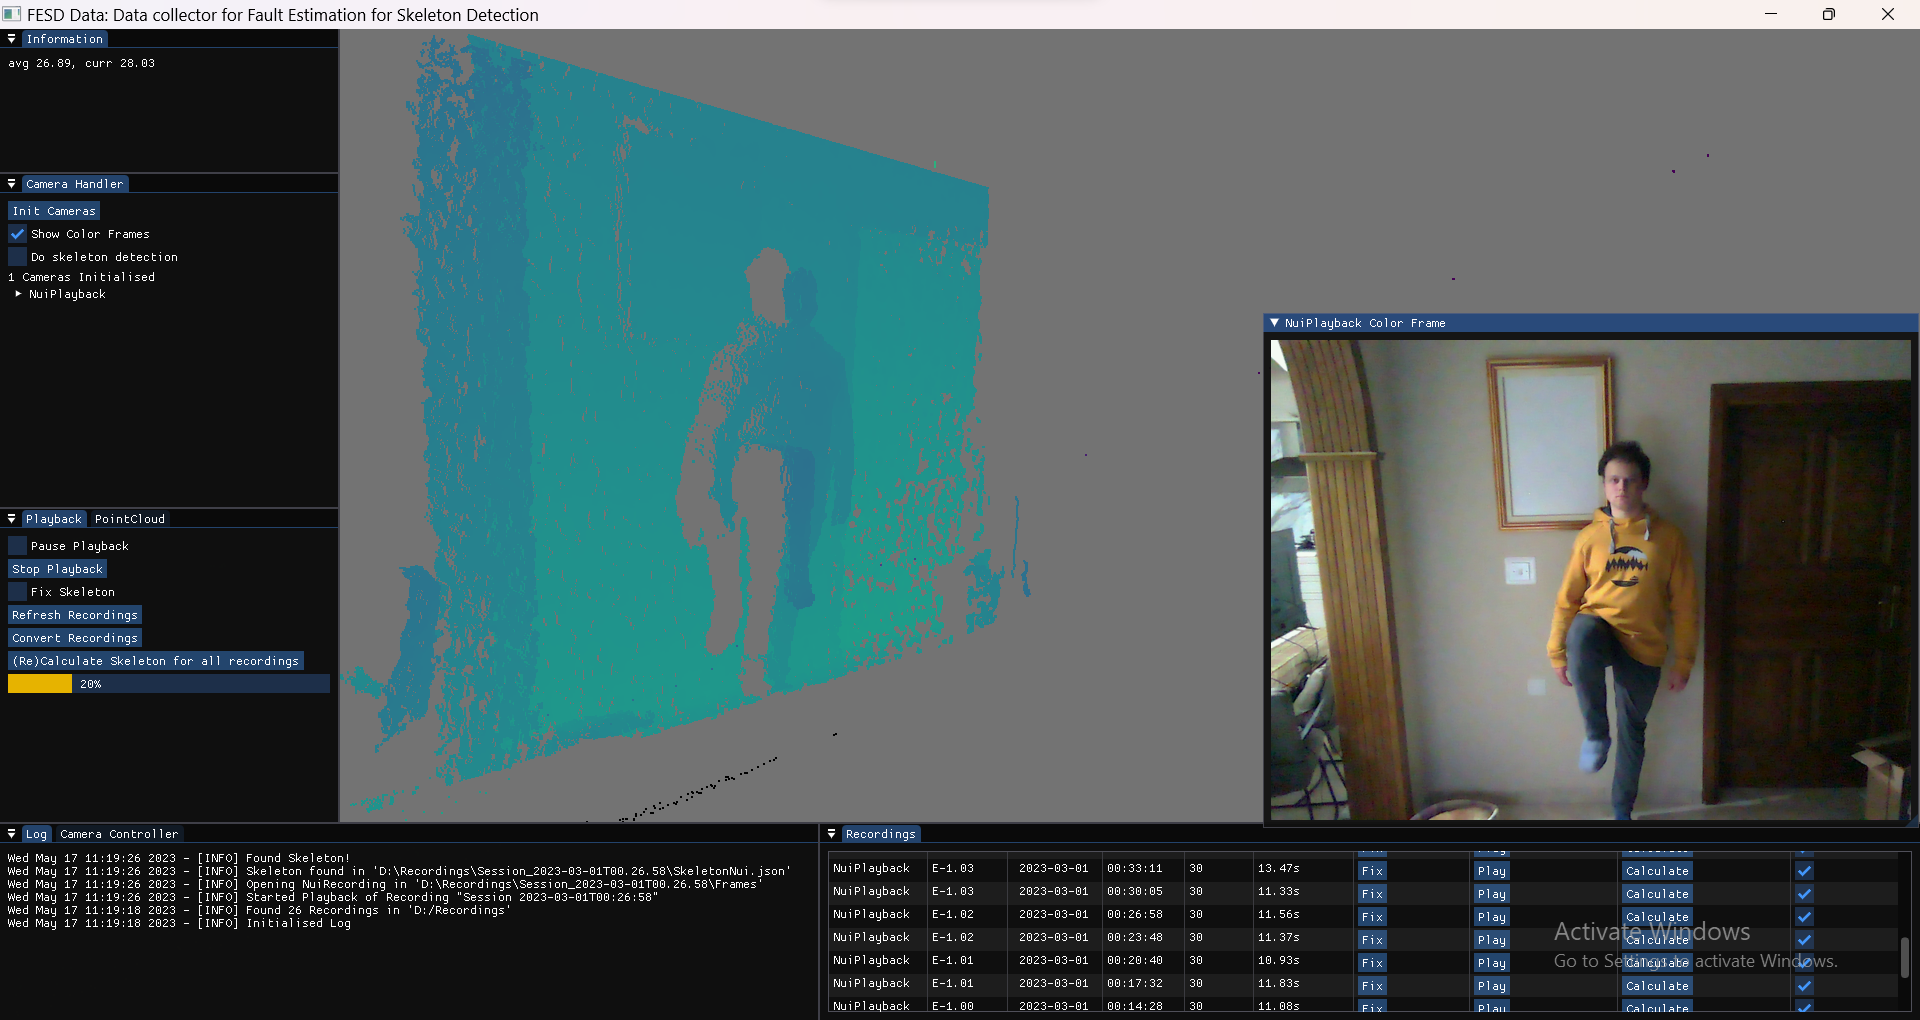
\includegraphics[width=\textwidth]{figures/FESDData/streaming.png}
  \end{subfigure}
  \hfill
  \begin{subfigure}[b]{0.49\linewidth}
      \centering
      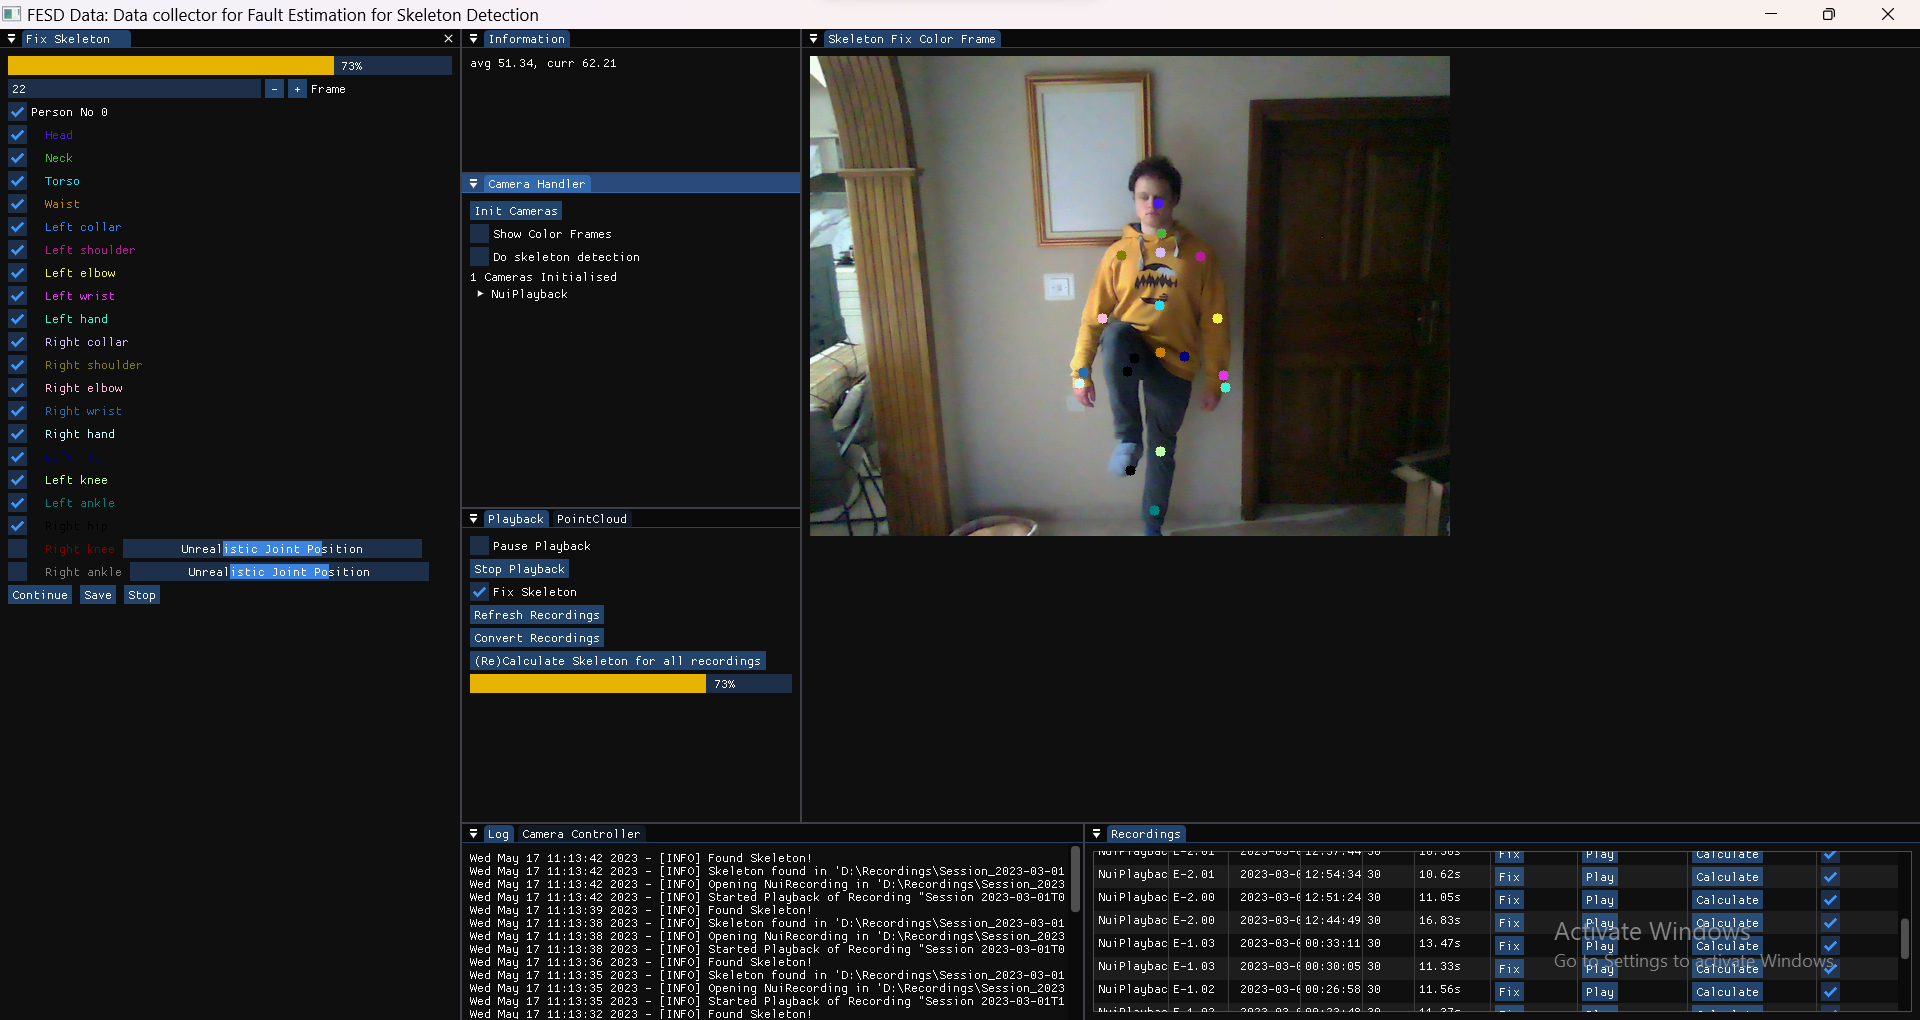
\includegraphics[width=\textwidth]{figures/FESDData/labelling.png}
  \end{subfigure}
  \caption[FESDData user interface]{A screenshot of the user interface with its two main components. On the left side, the user interface during streaming and recording can be seen and on the right side an example of data labelling.}
  \label{fig:fesddata}
\end{figure}  

\section{Data layout}

As mentioned earlier, the data is made up of multiple different streams or modalities. There are two separate visual streams, the RGB stream, and the depth stream, as well as the estimated human pose, the time stamps, and the recording metadata.

The visual streams are normalised and combined into a single file. OpenCV is used to store the RGB and the depth data into a single matrix and after the stream into a single file per frame. The RGB data is normalised to have values between 0 and 1, whereas the depth data is stored in meters.

The pose that is estimated by Nuitrack, as well as the error labels, are stored in a separate JSON file. The separate frames are stored in a list of frames. Each frame contains a list of all people that were detected. Each person contains a list of joints as well as an error label. Each joint is stored with real-world 3D coordinates which are stored in meters. These real-world coordinates are labelled $x$, $y$, and $z$. Additionally, the 2D projection and depth of the joint are stored in image coordinates and meters for the depth. The 2D projection is labelled $u$ and $v$ and the depth is labelled $d$. 

The error label is an integer which is the error id specific for joint and skeleton errors. The errors corresponding to the error ids are explained in section \ref{sec:data_labeling}. Finally, the timestamp of each frame is stored.

\subsection{Data labeling}
\label{sec:data_labeling}

A large part of the data preparation is the labelling of the data. The data is labelled with error labels. We define two different areas of errors. First, there are skeleton errors. Skeleton errors occur when the pose estimator detects a human in places where there are no humans. This can be caused by the pose estimator detecting a human in the background due to certain features that the estimator assumes are human.

Second, there are joint errors. Joint errors occur when the pose estimator detects a joint in the wrong place. This can be caused by the pose estimator detecting a joint in the background due to certain features that the estimator assumes are a joint. It can also be caused by the estimator labelling a joint incorrectly. 

For example, the estimator might label the left foot as the right foot. This is a common error, especially when the limbs are close too each other. An estimator might also not detect a joint at all. This might be caused through occlusion, be it by another joint, an object, or by the image border. Most applications avoid the last cause for occlusion by defining a minimum distance from the camera and specific camera placement to ensure that the user is always fully in view.

In the data, no error is denoted with $0$. If the whole skeleton is in a wrong position it can be labeled as faulty and subsequently every joint will be labeled with $2$. If a joint is not detected at all, it is labelled with $1$. If a joint is detected in the wrong place that is outside of the body, or somewhere where there should not be a joint, it is labelled with $2$. If a joint is detected in the approximate position of where another joint should be then it is labelled with $3$.

Implicitly, this creates two general labels, either a joint is faulty, i.e. the error label is $1$, $2$, or $3$, or it is not faulty, i.e. the error label is $0$. This makes the task easier, as it is a binary classification rather than a multi-class classification. However, we find the result to be enlightening as they might be more accurate and therefore more reliable.
\section{Dataset}

Multiple iterations of the recording process were run to find the best possible setup, which reduces the light interference as much as possible and which offers the best results with the resources at hand. The camera setup that is used by SilverFit was reproduced. At SilverFit the camera is mounted at $175cm$ above the floor. The camera that is used has an accelerometer which was used to adjust the camera angle relative to the ground. The camera is angled downward at a $70^\circ$ angle. 



% \subsection{Analysis}

% An important aspect of the dataset is the structure and distribution of data and their labels. In total, $REPLACE_WE$ recorded all 13 exercises, mentioned in Section \ref{sec:exercises}, twice. Each recording session consists of exactly 300 frames.

% If a joint cannot be detected by Nuitrack it automatically gets zero coordinates, i.e. every value is zero. This makes it easy to automatically label these joints as faulty, in particular with the error label $1$ - Joint Missing. However, for the rest of the errors each frame has to be manually inspected and each joint considered. Since this requires a lot of work $REPLACE_WE$ reduced the labeled frames to 10 percent of the original size. Therefore, each exercise contains 30 frames and in total $30 \cdot 13 \cdot 2 = 720$ frames are labeled.

% When multiple persons are detected one person might be incorrectly detected in the background. While analysing the data $REPLACE_WE$ pick the person that is not labeled as faulty whenever possible. For training and testing this is chosen at random. If a person is labeled as faulty each joint is marked as in an unrealistic position.

% \subsubsection{Distribution of Errors}

% An important factor in how well a model can be trained on data is the balance of the dataset. In this case, the dataset is balanced by the error labels. In Figure \ref{fig:statistics_err_dist} $REPLACE_WE$ can see the distribution of errors in the dataset as a whole. $REPLACE_WE$ see that most of the joints are not faulty, i.e. are in the position they are supposed be within a margin of error.

% \begin{figure}
%   \centering
%   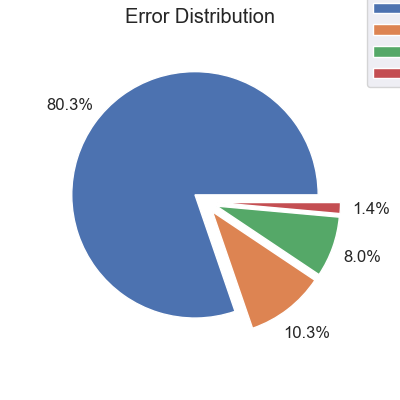
\includegraphics[width=0.5\textwidth]{figures/Data/Error_Distribution.png}
%   \caption[Error Distribution]{The distribution of errors TODO}
%   \label{fig:statistics_err_dist}
% \end{figure}

% To diversify the dataset $REPLACE_WE$ recorded different exercises with varying difficulties. In Figure \ref{fig:statistics_err_diff} $REPLACE_WE$ see that the difficulty has an influence on the amount of errors that occur for any given joint. $REPLACE_WE$ see that there is barely any difference between the trivial and the easy exercises. However, in Figure \ref{fig:statistics_err_dist_diff} $REPLACE_WE$ see that while trivial exercises have a higher percentage of unrealistic joint positions, i.e. the joint is in a wrong location, the easy exercises have a higher percentage of joints which are not detected. However, this difference is very small. Medium and Hard exercises are more error prone as was intended. This reflects $REPLACE_OUR$ design proposals for challenging exercises from Section \ref{sec:exercises} indeed cause more difficult scenarios.

% \begin{figure}
%   \centering
%   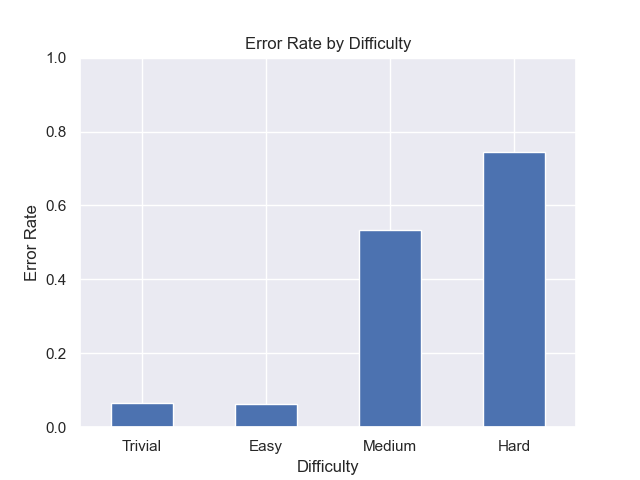
\includegraphics[width=0.5\textwidth]{figures/Data/Error_Rate_by_Difficulty.png}
%   \caption[Error Rate by Difficulty]{The rate that errors occur for any given difficulty. }
%   \label{fig:statistics_err_diff}
% \end{figure}

% \begin{figure}
%   \centering
%   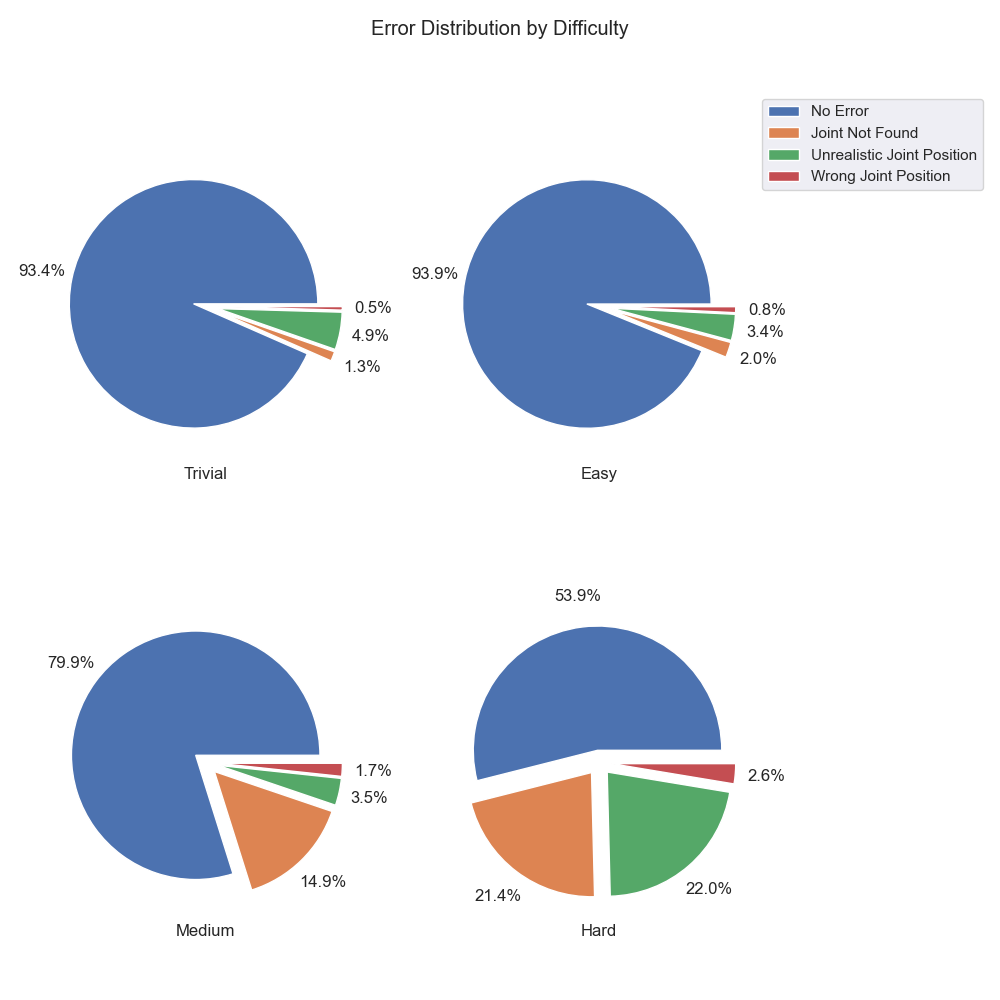
\includegraphics[width=0.5\textwidth]{figures/Data/Error_Distribution_by_Difficulty.png}
%   \caption[Error Distribution by Difficulty]{The distribution of errors by difficulty. TODO}
%   \label{fig:statistics_err_dist_diff}
% \end{figure}

% Some joints are more likely than others to be faulty, based on frequent occlusion, or generally more challenging detection. For example, hands and ankles are quite challenging to detect since they move frequently and are frequently occluded. On the other hand the head and the neck are least likely to be faulty. This distribution can be seen in Figure \ref{fig:statistics_err_dist_joint}, where the distribution of errors are shown for each joint. The joints are sorted by general occurrence of errors.

% \begin{figure}
%   \centering
%   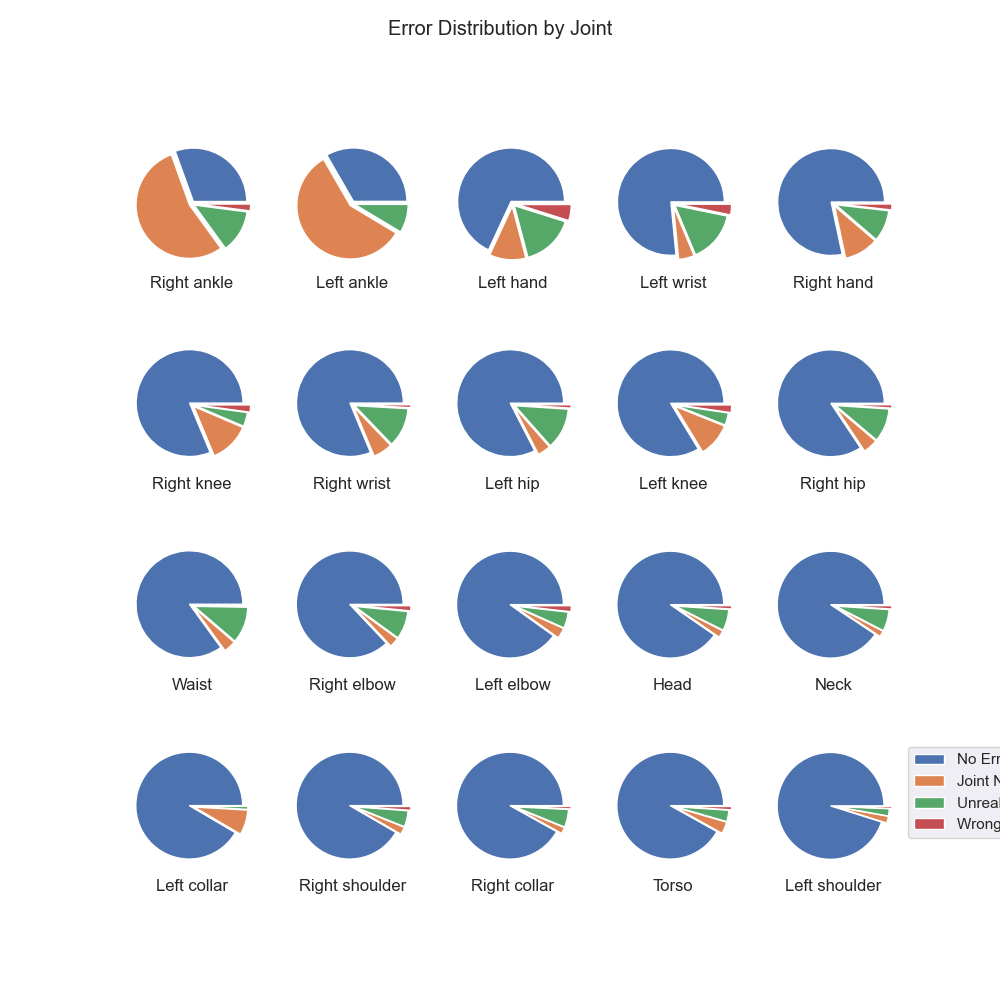
\includegraphics[width=0.5\textwidth]{figures/Data/Error_Distribution_by_Joint.png}
%   \caption[Error Distribution by Joint]{The distribution of errors by Joint. TODO}
%   \label{fig:statistics_err_dist_joint}
% \end{figure}

\subsection{Problem Sets}
\label{sec:problem_set}

Different problem sets are used to create different versions of the model. The problem sets are defined by the number of objects that are considered and are defined as erroneous. There are four different problem sets. The first problem set is the \textit{Joint} problem set. In this problem set, each joint is considered as a single object. The first simplification is to consider each joint, i.e. the individual arms, legs, torso, and head. The second simplification is to consider the upper and the lower body. Finally, only the whole body is considered.